\documentclass[dvipdfmx,11pt]{beamer}

%\usepackage{bxdpx-beamer}
\usepackage{listings,jlisting}
\usepackage{graphicx,xcolor} %文字の色
\usepackage[deluxe]{otf}
\usepackage{txfonts}


\usetheme{Warsaw}

\renewcommand{\kanjifamilydefault}{\gtdefault}
\renewcommand{\bibname}{参考文献}
\setbeamersize{text margin left=1.5em,text margin right=1.5em} %文字間の余白調整
\setbeamertemplate{navigation symbols}{} %アイコン消去
\setbeamertemplate{footline}[frame number] %フレーム番号表示
\useoutertheme{shadow}
\usefonttheme{professionalfonts} %数式文字のLaTeX化


\title{解集合プログラミングを用いたグラフ彩色問題の解法に関する考察}
\author{101830314 春田 穂高}
\institute{番原研究室}
\date{2021年度 卒業研究発表会\\2022年2月18日}

\begin{document}
%%%%%%%%%%%%%%%%%%%%%%%%%%%%%%%%%%%%%%%%%%%%%%%%%%%%%%%%%%%%%%%%%%%
\frame{\maketitle}
%%%%%%%%%%%%%%%%%%%%%%%%%%%%%%%%%%%%%%%%%%%%%%%%%%%%%%%%%%%%%%%%%%%

\begin{frame}{グラフ彩色問題と関連問題(1/2)}

 \begin{itemize}
  \item \alert{グラフ彩色問題}
        \begin{itemize}
         \item 与えられた有限無向グラフの隣接する頂点が,
               同色にならないように各頂点を彩色する際に,
               必要となる最小の色数を求める問題である.
         \item グラフ彩色問題はNP困難な問題である.
        \end{itemize}
  \item \alert{グラフ彩色判定問題}
        \begin{itemize}
         \item 与えられた有限無向グラフと色数に対して,
               グラフ彩色が可能かどうかを判定する問題である.
         \item グラフ彩色判定問題はNP完全な問題である.
        \end{itemize}
 \end{itemize}

 \begin{exampleblock}{グラフ彩色問題の応用}
  \begin{itemize}
   \item 最適化コンパイラのレジスタ割り付け
   \item 無線の周波数割り当て
  \end{itemize}
  
 \end{exampleblock}
 
\end{frame}

%%%%%%%%%%%%%%%%%%%%%%%%%%%%%%%%%%%%%%%%%%%%%%%%%%%%%%%%%%%%%%%%%%%

\begin{frame}{グラフ彩色問題と関連問題(2/2)}

 \begin{itemize}
  \item \alert{グラフ彩色における同色頂点数最小化問題}
        \begin{itemize}
         \item グラフ彩色問題において,同色で彩色する頂点数を最小化する問題である.
        \end{itemize}
  \item \alert{グラフ彩色における同色頂点数最大化問題}
        \begin{itemize}
         \item グラフ彩色問題において,同色で彩色する頂点数を最大化する問題である.
        \end{itemize}
  \item \alert{グラフ彩色における多色頂点数最大化問題}
        \begin{itemize}
         \item グラフ彩色問題において,2色以上で彩色できる頂点数を最大化する問題である.
        \end{itemize}
 \end{itemize}
 
 \begin{alertblock}{}
  本研究では,グラフ彩色判定問題とその関連問題を対象とする.
 \end{alertblock}
 
\end{frame}

%%%%%%%%%%%%%%%%%%%%%%%%%%%%%%%%%%%%%%%%%%%%%%%%%%%%%%%%%%%%%%%%%%%

\begin{frame}{McGregorグラフ}
 \begin{exampleblock}{order5のMcGregorグラフ}
  \begin{center}
   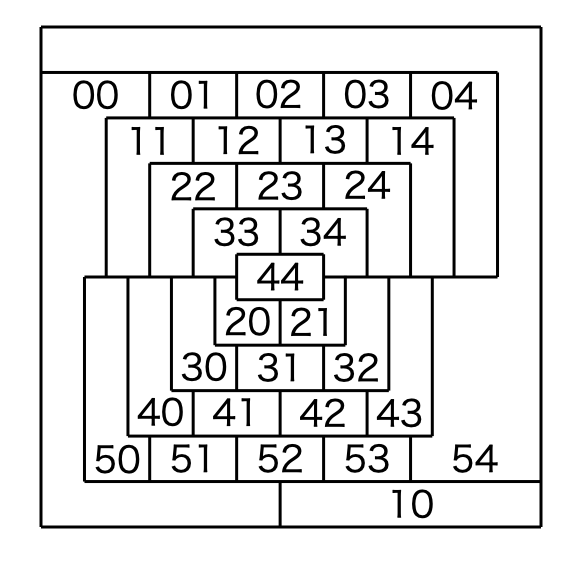
\includegraphics[scale=0.2]{fig/order5.png}
  \end{center}
  % \begin{itemize}
  %  \item 頂点数: 30
  %  \item 辺数: 84
  % \end{itemize}
 \end{exampleblock}

 \begin{itemize}
  \item D.~E~.Knuthの教科書
         The Art of Computer Programming~\cite{Knuth:TAOCP:SAT}
         に記載されているグラフである.
  \item McGregorグラフは4彩色可能なグラフである.
  \item 頂点数,辺数はorder(=n)のサイズによって決まる.
 \end{itemize}
 
\end{frame}

%%%%%%%%%%%%%%%%%%%%%%%%%%%%%%%%%%%%%%%%%%%%%%%%%%%%%%%%%%%%%%%%%%%

\begin{frame}{多色頂点数最大化問題の例}

 \begin{exampleblock}{order5のMcGregorグラフ\cite{Knuth:TAOCP:SAT}}
  \begin{tabular}{cc}
   \begin{minipage}[t]{0.5\linewidth}
    \centering
    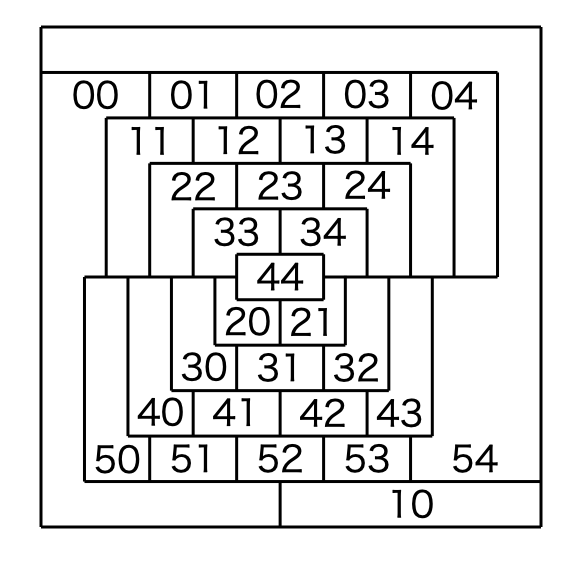
\includegraphics[scale=0.2]{fig/order5.png}
   \end{minipage}
   \begin{minipage}[t]{0.5\linewidth}
    \centering
    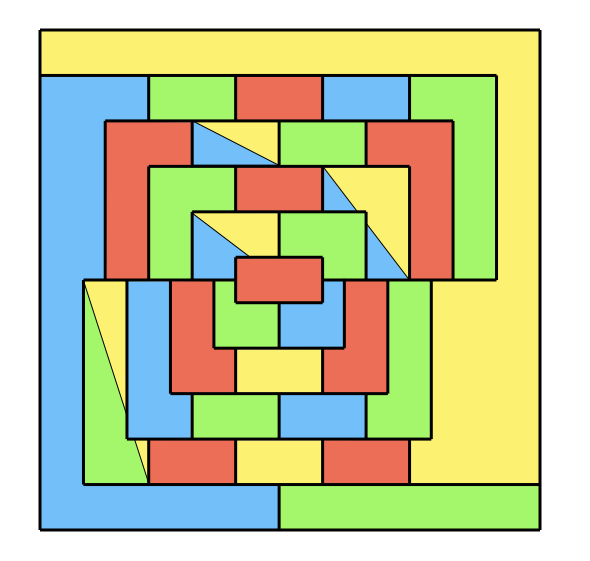
\includegraphics[scale=0.2]{fig/order5_mult.png}
   \end{minipage}
  \end{tabular}
 \end{exampleblock}

 \begin{alertblock}{}
  \begin{itemize}
   \item 頂点番号12,24,33,50が多色で彩色できる.
   \item $2^4=$\alert{\textbf{16}}通りの彩色の組み合わせを表している.
  \end{itemize}
 \end{alertblock}

\end{frame}

%%%%%%%%%%%%%%%%%%%%%%%%%%%%%%%%%%%%%%%%%%%%%%%%%%%%%%%%%%%%%%%%%%%

\begin{frame}{解集合プログラミング(Answer Set Programming; ASP)}

 \begin{itemize}
  \item \alert{ASP}は,論理プログラミングから派生した
        比較的新しいプログラミングパラダイムである.
  \item \alert{ASP言語}は,一階論理に基づいた知識表現言語の一種である.
  \item \alert{ASPシステム}は,論理プログラムから
        安定モデル意味論~{\scriptsize[Gelfond and Lifschitz, '88]}
        に基づく解集合を計算するシステムである.
  \item 近年,SAT技術を利用する高速なASPシステムが開発され,
        様々な分野への実用的な応用が急速に拡大している.
 \end{itemize}
 
 \begin{alertblock}{グラフ彩色判定問題に対してASPを用いる利点}
  \begin{itemize}
   \item ASP言語の高い表現力により,制約を簡潔に記述可能.
   \item 充足不能コアを用いた最適化探索が可能.
   \item 高速ASPシステムを用いた高速な解探索,解列挙が可能.
  \end{itemize}
 \end{alertblock}
 
\end{frame}

%%%%%%%%%%%%%%%%%%%%%%%%%%%%%%%%%%%%%%%%%%%%%%%%%%%%%%%%%%%%%%%%%%%

\begin{frame}{研究目的と内容}

 \begin{alertblock}{研究目的}
  \begin{itemize}
   \item グラフ彩色判定問題とその関連問題に対して,
         ASP符号化を提案し,評価する.
   \item 得られた解を利用した,グラフ彩色問題の実行可能解の圧縮.
  \end{itemize}

 \end{alertblock}

 \begin{block}{研究内容}
  \begin{enumerate}
   \item \structure{グラフ彩色判定問題とその関連問題を解くASP符号化の提案}
         \begin{itemize}
          \item color符号化,minimize符号化,
                maximize符号化,mult符号化.
         \end{itemize}
   \item \structure{ベンチマーク問題を用いた評価実験}
         \begin{itemize}
          \item McGregorグラフを138問,新たに作成.
          \item グラフ彩色判定問題とその関連問題に対する実験.
         \end{itemize}
   \item \alert{グラフ彩色問題の実行可能解の圧縮}
         \begin{itemize}
          \item mult符号化で得られる解が基のグラフ彩色問題の
                実行可能解の何通りを表しているかの調査.
         \end{itemize}
   \item \structure{グラフ彩色問題の実行可能解の全解列挙}
  \end{enumerate}
 \end{block}
 
\end{frame}

%%%%%%%%%%%%%%%%%%%%%%%%%%%%%%%%%%%%%%%%%%%%%%%%%%%%%%%%%%%%%%%%%%%

\begin{frame}{提案するASP符号化}

 \begin{block}{ASP符号化}
 各問題に対してASP符号化を提案した.

 \begin{enumerate}
  \item \alert{color符号化}(グラフ彩色判定問題):
        \begin{itemize}
         \item ASPの個数制約を用いて簡潔に記述.
        \end{itemize}
  \item \alert{minimize符号化}(同色頂点数最小化問題):
        \begin{itemize}
         \item color符号化をベースに
               ASPの最小化関数を用いて簡潔に記述.
        \end{itemize}
  \item \alert{maximize符号化}(同色頂点数最大化問題):
        \begin{itemize}
         \item color符号化をベースに
               ASPの最大化関数を用いて簡潔に記述.
        \end{itemize}
  \item \alert{mult符号化}(多色頂点数最大化問題):
        \begin{itemize}
         \item color符号化をベースに
               頂点を彩色する色の数をASPの個数制約を用いて変更.
         \item ASPの最大化関数を用いて多色で彩色できる頂点数を最大化するよう記述.
        \end{itemize}
 \end{enumerate}
 \end{block}
\end{frame}

%%%%%%%%%%%%%%%%%%%%%%%%%%%%%%%%%%%%%%%%%%%%%%%%%%%%%%%%%%%%%%%%%%%

\begin{frame}{実験概要}
 \begin{block}{}
  提案する符号化の有効性を評価するため,実験を行った.
 \end{block}

 \begin{block}{}
  \begin{itemize}
   \item \structure{ベンチマーク問題}: McGregorグラフのorder3$\sim$140までの138問
   \item \structure{ASPシステム}: \textit{clingo}-5.5.0
   \item \structure{実験環境}: Mac mini Intel Core i7 3.2GHz 64GBメモリ
   \item \structure{制限時間}: 
         \begin{itemize}
          \item color符号化: 30分
          \item minimize,maximize,mult符号化: 1時間
         \end{itemize}
  \end{itemize}  
 \end{block}

 \begin{alertblock}{color符号化の実験結果}
  order3$\sim$138の計136問について彩色できることがわかった.
 \end{alertblock}
 
\end{frame}

%%%%%%%%%%%%%%%%%%%%%%%%%%%%%%%%%%%%%%%%%%%%%%%%%%%%%%%%%%%%%%%%%%%

\begin{frame}{実験結果:同色頂点数最小化問題}

 \begin{block}{}
  \structure{問題数}: order3$\sim$20までの18問
 \end{block}

 \begin{center}
  \begin{tabular}{r|c|c}
 %n& f(n)\\
 N&BB &USC\\
 \hline
 3&2*&2*\\
 4&2*&2*\\
 5&3*&3*\\
 6&4*&4*\\
 7&5*&5*\\
 8&7*&7*\\
 9&7*&7*\\
 10&7*&7*\\
 11&8*&8*\\
 12&9*&9*\\
 13&10*&10*\\
 14&12&\textbf{12*}\\
 15&\textbf{12}&49\\
 16&16&\textbf{12*}\\
 17&21&\textbf{\textcolor{red}{13*}}\\
 18&19&\textbf{\textcolor{red}{14*}}\\
 19&\textbf{20}&58\\
 20&\textbf{22}&59\\\hline
\end{tabular}


 \end{center}

 \begin{itemize}
  \item BB法とUSC法ではUSC法の方が良い結果を得られた.
  \item order3$\sim$14,16$\sim$18問の計15問について最適値を求めることができた.
  \item 新たに2問について最適値を発見することができた.
 \end{itemize}
 
\end{frame}

%%%%%%%%%%%%%%%%%%%%%%%%%%%%%%%%%%%%%%%%%%%%%%%%%%%%%%%%%%%%%%%%%%%

\begin{frame}{実験結果:同色頂点数最大化問題}

 \begin{block}{}
  \structure{問題数}: order3$\sim$38までの36問
 \end{block}
 
 \begin{center}
  \begin{table}[t]\scriptsize
%\renewcommand{\arraystrech}{1.2}
\begin{tabular}{r|cc||r|cc||r|cc}
 \hline
 %n& g(n)\\
 N&BB &USC&N&BB&USC&N&BB&USC\\
 \hline
 3&4*&4*&    15&71&\textbf{77*}&
 27&\textbf{185}&180 \\
 4&6*&6*&    16&71&\textbf{88*}&
 28&199&\textbf{\textcolor{red}{266*}} \\
 5&10*&10*&    17&76&\textbf{\textcolor{red}{99*}}&
 29&221&\textbf{\textcolor{red}{285*}} \\
 6&13*&13*&    18&91&\textbf{\textcolor{red}{111*}}&
 30&224&\textbf{\textcolor{red}{305*}} \\
 7&17*&17*&    19&92&\textbf{\textcolor{red}{123*}}&
 31&247&\textbf{\textcolor{red}{325*}} \\
 8&23*&23*&    20&109&\textbf{\textcolor{red}{137*}}&
 32&255&255 \\
 9&28&\textbf{28*}&    21&121&\textbf{\textcolor{red}{150*}}&
 33&\textbf{280}&278 \\
 10&35&\textbf{35*}&    22&122&\textbf{\textcolor{red}{165*}}&
 34&296&\textbf{\textcolor{red}{391*}} \\
 11&42&\textbf{42*}&    23&137&\textbf{\textcolor{red}{180*}}&
 35&310&\textbf{\textcolor{red}{414*}} \\
 12&49&\textbf{50*}&    24&146&\textbf{\textcolor{red}{196*}}&
 36&338&\textbf{\textcolor{red}{438*}} \\
 13&56&\textbf{58*}&    25&162&\textbf{\textcolor{red}{212*}}&
 37&\textbf{348}&340 \\
 14&56&\textbf{68*}&    26&180&\textbf{\textcolor{red}{230*}}&
 38&371&371 \\ 
\end{tabular}
\end{table}

 \end{center}

 \begin{itemize}
  \item BB法とUSC法ではUSC法の方が良い結果を得られた.
  \item USC法が31問について最適値を求めることができた.
  \item 新たに17問について最適値を発見することができた.
 \end{itemize}

\end{frame}

%%%%%%%%%%%%%%%%%%%%%%%%%%%%%%%%%%%%%%%%%%%%%%%%%%%%%%%%%%%%%%%%%%%

\begin{frame}{実験結果:多色頂点数最大化問題}

 \begin{block}{}
  \structure{問題数}: order3$\sim$15までの13問
 \end{block}
 
 \begin{center}
  \begin{tabular}{r|r|r}
 %n& h(n)\\
 N&BB &USC\\
 \hline
 3&1*&1*\\
 4&3*&3*\\
 5&4*&4*\\
 6&7*&7*\\
 7&9*&9*\\
 8&13*&13*\\
 9&18*&18*\\
 10&23&\textbf{23*}\\
 11&27&\textbf{\textcolor{red}{29*}}\\
 12&34&\textbf{\textcolor{red}{36*}}\\
 13&\textbf{39}&15\\
 14&\textbf{44}&11\\
 15&\textbf{49}&20\\\hline
\end{tabular}


 \end{center}

 \begin{itemize}
  \item BB法とUSC法ではUSC法の方が良い結果を得られた.
  \item USC法が10問について最適値を求めることができた.
  \item 新たに2問について最適値を発見することができた.
 \end{itemize}

\end{frame}

%%%%%%%%%%%%%%%%%%%%%%%%%%%%%%%%%%%%%%%%%%%%%%%%%%%%%%%%%%%%%%%%%%%

\begin{frame}{実行可能解の圧縮}

 \begin{block}{}
  多色頂点数最大化問題の実験で得られた解が,
  基のグラフ彩色問題の実行可能解の何通りを表しているかを調査した.
 \end{block}
 
 \begin{center}
  \begin{tabular}{r|c|c|c}
 \hline
 n& h(n)& 圧縮された解の個数& 圧縮率 \\
 \hline
 3&	1&	2&	1.3889 \\
 4&	3&	8&	0.3367 \\
 5&	4&	16&	0.0368 \\
 6&	7&	128&	0.0049 \\
 7&	9&	512&	0.0002 \\
 8&	13&	8192&	- \\
 9&	18&	262144&	- \\
 10&	23&	8388608&	- \\
 11&	29&	536870912&	- \\
 12&	36&	68719476736&	- \\
\end{tabular}
\caption{多色頂点数最大化問題の解の圧縮率}
\label{table:com}
 \end{center}

 \begin{itemize}
  \item 多色頂点数最大化問題で最適値を発見できた
        order3$\sim$12までの計10問の解の圧縮に成功した.
  \item order12では約680億もの実行可能解を表していることがわかった.
 \end{itemize}

\end{frame}

%%%%%%%%%%%%%%%%%%%%%%%%%%%%%%%%%%%%%%%%%%%%%%%%%%%%%%%%%%%%%%%%%%%

\begin{frame}{まとめと今後の課題}

 \begin{enumerate}
  \item \structure{グラフ彩色判定問題とその関連問題を解くASP符号化の提案}
        \begin{itemize}
         \item ASPの高い表現力により簡潔に記述できることが確認できた.
        \end{itemize}
  \item \structure{McGregorグラフを用いた評価実験}
        \begin{itemize}
         \item 各問題に対して,新たに最適値を発見することに成功した.
        \end{itemize}
  \item \structure{グラフ彩色問題の実行可能解の圧縮}
        \begin{itemize}
         \item 多色頂点数最大化問題で発見した10問について
               解の圧縮することに成功した.
        \end{itemize}
  \item \structure{グラフ彩色問題の実行可能解の全解列挙}
 \end{enumerate}

 \begin{block}{今後の課題}
  \begin{itemize}
   \item ASP符号化の改良
   \item McGregorグラフ以外のグラフでの評価実験
  \end{itemize}
 \end{block}
 
\end{frame}

%%%%%%%%%%%%%%%%%%%%%%%%%%%%%%%%%%%%%%%%%%%%%%%%%%%%%%%%%%%%%%%%%%%

\begin{frame}[noframenumbering]{参考文献}
 \bibliographystyle{jplain} % 参考文献スタイル
 \bibliography{aisat,bachelor}    % 参考文献リスト
\end{frame}

%%%%%%%%%%%%%%%%%%%%%%%%%%%%%%%%%%%%%%%%%%%%%%%%%%%%%%%%%%%%%%%%%%%

\begin{frame}[noframenumbering]{}
 \thispagestyle{empty}
 \Huge 付録
\end{frame}

%%%%%%%%%%%%%%%%%%%%%%%%%%%%%%%%%%%%%%%%%%%%%%%%%%%%%%%%%%%%%%%%%%%

\begin{frame}[noframenumbering]{グラフ彩色問題の実行可能解の全解列挙(1/2)}
 \thispagestyle{empty}

 \begin{block}{}
  %グラフ彩色における多色頂点数最大化問題の実行可能解の圧縮を確認するために,
  グラフ彩色問題の実行可能解の全解列挙する実験を行った.  
 \end{block}

 \begin{block}{実験概要}
  \begin{itemize}
   \item \structure{ASPシステム}: \textit{clingo}-5.5.0
   \item \structure{実験環境}: Mac mini Intel Core i7 3.2GHz 64GBメモリ
   \item \structure{制限時間}: 1時間
   \item \structure{問題数}: McGregorグラフのorder3$\sim$10までの計8問
  \end{itemize}
 \end{block}
\end{frame}

%%%%%%%%%%%%%%%%%%%%%%%%%%%%%%%%%%%%%%%%%%%%%%%%%%%%%%%%%%%%%%%%%%%

\begin{frame}[noframenumbering]{グラフ彩色問題の実行可能解の全解列挙(2/2)}
 \thispagestyle{empty}

 \begin{center}
  \begin{tabular}{r|r|r}
 \hline
 N& 解の総数& CPU時間\\
 3&144*&0.002\\
 4&2376*&0.009\\
 5&43536*&0.143\\
 6&2589768*&7.796\\
 7&224442336*&865.500\\
 8&$\geq$816623222&-\\
 9&$\geq$676088853&-\\
 10&$\geq$504392039&-\\
\end{tabular}

 \end{center}

 \begin{itemize}
  \item order3$\sim$7までの計5問について全解列挙に成功した.
 \end{itemize}
\end{frame}

%%%%%%%%%%%%%%%%%%%%%%%%%%%%%%%%%%%%%%%%%%%%%%%%%%%%%%%%%%%%%%%%%%%
\end{document}

%%% Local Variables:
%%% mode: japanese-latex
%%% TeX-master: 
%%% End: